%% IEEE Double-Column Conference Paper Format
\documentclass[10pt,twocolumn]{article}
\usepackage[margin=0.75in]{geometry}
\usepackage{cite}
\usepackage{amsmath,amssymb,amsfonts}
\usepackage{graphicx}
\usepackage{textcomp}
\usepackage{xcolor}
\usepackage{booktabs}
\usepackage{url}
\usepackage{times}

% IEEE-style title
\makeatletter
\renewcommand{\maketitle}{%
  \twocolumn[
    \begin{@twocolumnfalse}
      \begin{center}
        {\LARGE\bfseries \@title \par}
        \vskip 1em
        {\large \@author \par}
        \vskip 0.5em
      \end{center}
    \end{@twocolumnfalse}
  ]
}
\makeatother

\begin{document}

\title{\textbf{Comparing Tree Ensembles and Deep Learning for Network Intrusion Detection on Imbalanced Data}}

\author{
Mohammed Abdul Razzak Baig \\
MSc Machine Learning, National College of Ireland \\
Student ID: 25207938
}

\maketitle

\begin{abstract}
Production network intrusion detection confronts a challenging reality: benign traffic comprises over 80\% of observations, while critical attack categories contain fewer than 100 labeled examples. Despite widespread enthusiasm for neural architectures, their effectiveness under such extreme imbalance remains empirically unverified. We conduct a rigorous controlled study comparing tree-based learners (Random Forest, XGBoost) against a 1D convolutional network on CICIDS2017, measuring both predictive performance and operational feasibility. Our findings reveal XGBoost achieving 85.55\% macro-F1 versus CNN's 61.13\%---a 24-point performance differential. Analysis uncovers a pivotal 100-example boundary: tree models exhibit graceful degradation (60--70\% F1) below this threshold, while the CNN experiences complete failure (0--40\% F1). From a deployment perspective, XGBoost trains in 8 minutes, consumes 50 MB storage, and processes flows in 30 ms on commodity CPUs. These results question prevailing assumptions about neural network supremacy for tabular intrusion detection under severe imbalance.
\end{abstract}

\textbf{Keywords:} Network Intrusion Detection, Imbalanced Learning, Deep Learning, Tree Ensembles, XGBoost, CNN, CICIDS2017

\section{Introduction}

Automated detection of malicious network activity represents a cornerstone capability for organizational cybersecurity, with annual damages from breaches projected to exceed \$10.5 trillion by 2025 \cite{cybercrime2025}. A distinctive characteristic of this domain is extreme distributional skew: legitimate communications typically account for 80--90\% of observed flows, while sophisticated threats such as zero-day exploits or advanced persistent threats may surface in under 10 training instances.

Three substantial methodological shortcomings pervade contemporary literature. The prevalence of accuracy-centric reporting creates misleading impressions---trivially predicting "benign" for all observations yields 99\% accuracy despite detecting zero attacks. Operational considerations including computational overhead, storage footprint, and inference speed receive minimal attention, despite determining real-world viability. Performance on minority attack categories is frequently excluded or selectively presented, masking actual detection capabilities where it matters most.

Neural architectures enjoy considerable presumed superiority, yet rigorous empirical validation under severe imbalance remains absent. Meanwhile, ensemble decision tree methods \cite{breiman2001random,chen2016xgboost} demonstrate documented effectiveness on skewed distributions, though direct head-to-head comparisons using standardized protocols are missing. We address this gap by investigating two core questions:

\textbf{RQ1:} Do convolutional networks achieve parity with tree ensembles on sparse attack categories under class-balanced evaluation?

\textbf{RQ2:} Which architecture delivers optimal trade-offs between predictive quality and operational requirements?

Our central hypothesis posits that tree-based methods exhibit superior sample efficiency---requiring fewer labeled examples to achieve equivalent performance (Fig. \ref{fig:comparison}).

\textbf{Contributions:} We deliver (1) rigorous controlled evaluation using identical data and protocols, (2) joint assessment of detection quality and deployment feasibility, (3) discovery of a critical 100-sample inflection point, (4) detailed failure mode analysis across architectures, and (5) concrete deployment recommendations for practitioners.

\section{Related Work}

\subsection{Network Intrusion Detection}

Early intrusion detection relied on signature matching—pattern databases identifying known threats. Machine learning approaches emerged as an alternative, replacing manual rule curation with statistical learning \cite{buczak2016survey}. CICIDS2017 \cite{sharafaldin2018cicids} has achieved benchmark status, appearing in over 50 publications. A persistent methodological flaw undermines many studies: accuracy-centric reporting masks detection failures. Classifying all observations as benign yields 84.94\% accuracy despite zero threat identification. This "accuracy mirage" inflates apparent performance while obscuring practical capabilities.

Evaluation protocols frequently exclude sparse attack categories, reporting metrics only for classes exceeding 1000 training examples. Such selective reporting conceals performance precisely where detection matters most—novel, infrequent threats. Our evaluation encompasses all 15 categories, including transparent reporting of architectural shortcomings.

\subsection{Deep Learning for NIDS}

Neural architectures have attracted substantial interest for intrusion detection. Ferrag et al. \cite{ferrag2020deep} synthesized deep learning approaches, identifying convolutional, recurrent, transformer, and hybrid designs. CNNs extract spatial feature patterns, RNNs model temporal dependencies, autoencoders perform unsupervised anomaly identification. However, these investigations typically exhibit: (1) accuracy as evaluation priority, (2) absent deployment analysis, (3) omission of per-category sparse class metrics.

Contemporary work explores attention mechanisms and transformer architectures, claiming performance advantages. Yet these comparisons employ disparate datasets, preprocessing protocols, and evaluation frameworks, precluding objective assessment. Our investigation provides standardized comparison where all architectures train on identical data under uniform conditions.

\subsection{Imbalanced Learning}

He and Garcia \cite{he2009imbalanced} taxonomize imbalanced learning into data-level (resampling) and algorithm-level (cost-sensitive) interventions. Data-level approaches encompass minority oversampling (SMOTE \cite{chawla2002smote}), majority undersampling, or hybrid strategies. SMOTE synthesizes artificial minority examples, potentially creating non-representative patterns that induce overfitting on manufactured data.

Algorithm-level methods modify objective functions or category weights. Focal Loss \cite{lin2017focal} diminishes well-classified example contributions, concentrating learning on challenging cases. This proved effective for object detection with 1:1000 imbalance ratios. Class-balanced loss adaptively modulates weights based on effective sample counts. Our CNN employs Focal Loss with square-root class weighting, representing current best practices for neural imbalanced learning. Despite this optimization, it underperforms tree ensembles by 24 points, indicating fundamental architectural limitations transcending loss function selection.

\subsection{Tree Ensembles vs. Deep Learning}

Tree-based ensembles demonstrate robust performance on skewed NIDS distributions. Random Forests achieve robustness through bootstrap aggregation, while XGBoost amplifies signal via gradient boosting. Sample efficiency emerges from localized learning: individual tree nodes learn from feature space subregions, maintaining effectiveness despite sparse overall category representation.

Published comparisons yield conflicting conclusions. Some report tree ensemble superiority on CICIDS2017, but employ divergent preprocessing, partitioning, and metrics. Others claim deep learning advantages, but utilize aggressive data augmentation or exclude sparse categories. Absent controlled evaluation, relative merits remain ambiguous. This investigation addresses that gap.


\section{Methodology}

\subsection{Dataset}

We employ CICIDS2017 \cite{sharafaldin2018cicids}, comprising 2,830,743 bidirectional flow observations captured across five consecutive days (July 3--7, 2017) within an emulated enterprise network. This corpus encompasses typical organizational activities (HTTP browsing, SMTP communication, FTP transfers) alongside 14 adversarial scenarios executed by security professionals: distributed denial-of-service, port reconnaissance, botnet traffic, credential stuffing (FTP/SSH), application-layer DoS variants (Slowloris, Slowhttptest, Hulk, GoldenEye), SSL vulnerability exploitation (Heartbleed), and web application attacks (brute force, cross-site scripting, SQL injection, infiltration).

CICFlowMeter extracts 77 statistical descriptors per flow, organized across dimensions:
\begin{itemize}
    \item \textbf{Volumetric:} Duration, packet count, byte volume
    \item \textbf{Timing:} Inter-arrival time moments (mean, variance, extrema)
    \item \textbf{Asymmetry:} Forward/backward packet/byte asymmetry, bulk transfer rates
    \item \textbf{Distributional:} Packet length moments, flow inter-arrival statistics
    \item \textbf{Control plane:} TCP flags (FIN, SYN, RST, PSH, ACK, URG), header dimensions
\end{itemize}

The core challenge emerges from distributional skew. Table \ref{tab:distribution} quantifies the imbalance: 84.94\% legitimate flows, with adversarial categories spanning 9.60\% (DDoS) down to 0.0003\% (Heartbleed). Six categories contain under 100 training examples; the sparsest (Botnet ARES) presents merely 8 instances. This extreme skew authentically reflects operational environments where threats constitute rare events.

\begin{table}[htbp]
\caption{CICIDS2017 Class Distribution (Top 10)}
\label{tab:distribution}
\centering
\small
\begin{tabular}{lrc}
\toprule
\textbf{Class} & \textbf{Samples} & \textbf{Percentage} \\
\midrule
BENIGN & 2,273,097 & 84.94\% \\
DDoS & 256,612 & 9.60\% \\
PortScan & 182,103 & 6.79\% \\
Bot & 30,353 & 1.13\% \\
FTP-Patator & 9,522 & 0.36\% \\
SSH-Patator & 7,076 & 0.26\% \\
DoS Hulk & 2,774 & 0.10\% \\
DoS GoldenEye & 1,230 & 0.05\% \\
Infiltration & 970 & 0.04\% \\
DoS Slowloris & 939 & 0.04\% \\
\bottomrule
\end{tabular}
\end{table}

\subsection{Preprocessing Pipeline}

Data preparation follows systematic protocols ensuring integrity and generalizability:

\textbf{Deduplication:} Preliminary analysis identified 596,780 exact replicas (21.06\% of corpus), stemming from temporal overlap across daily capture files. Elimination yields 2,233,963 unique observations, preventing evaluation contamination.

\textbf{Missing Value Treatment:} Absent values affect 0.03\% of flows, concentrated in reverse-direction metrics for unidirectional communications. Median-based imputation within feature families preserves distributional characteristics without introducing systematic bias.

\textbf{Information Leakage Mitigation:} Several attributes provide trivial classification shortcuts unsuitable for deployment:
\begin{itemize}
    \item \textbf{Destination Port:} Exhibits perfect correlation with attack categories (SSH intrusions target port 22, FTP attacks port 21). Removal compels behavioral pattern learning rather than port memorization.
    \item \textbf{Bwd PSH Flags:} Systematically zero for unidirectional attacks, enabling trivial discrimination.
    \item \textbf{Init Fwd Win Bytes, Fwd Header Length:} Correlated with specific penetration testing tools, undermining cross-environment generalization.
\end{itemize}

Leak mitigation induces 2--3\% accuracy reduction but ensures learned representations transfer beyond dataset artifacts.

\textbf{Feature Scaling:} The surviving 73 attributes undergo z-score transformation: $x' = \frac{x - \mu}{\sigma}$, with moments $\mu, \sigma$ computed exclusively from training data. This centering and scaling prevents magnitude-driven feature dominance.

\subsection{Train/Validation/Test Split}

Data was split 70\%/15\%/15\% into training (1,563,774 samples), validation (335,094 samples), and test (335,095 samples) sets using stratified sampling. Stratification preserves class ratios across splits, ensuring rare attacks appear in all three sets. For classes with <10 samples, we manually verified at least 1 sample appears in each set. The validation set enables hyperparameter tuning without touching the test set, preventing optimistic bias.

\subsection{Model Architectures}

\textbf{Random Forest:} We train an ensemble of 500 decision trees using bootstrap aggregating (bagging). Each tree trains on a random 63\% sample of training data (bootstrap sample) and considers $\sqrt{n} \approx 9$ randomly selected features per split decision. Trees grow without depth limit until nodes are pure or contain <5 samples. The Gini impurity criterion guides splits: $G = 1 - \sum_{i=1}^{C} p_i^2$, where $p_i$ is the proportion of class $i$ at the node. Class weights are balanced as $w_i = \frac{n_{samples}}{n_{classes} \cdot n_{samples\_i}}$ to penalize majority class errors. Implementation uses scikit-learn 1.0.2 with n\_jobs=-1 for parallel training across all CPU cores. Training time: 15 minutes on 16-core Xeon CPU. Model size: 294 MB (pickled).

\textbf{XGBoost:} We employ gradient boosting with 300 sequential trees. Each new tree corrects residual errors from the ensemble so far. Learning rate $\eta=0.1$ controls the contribution of each tree, preventing overfitting through shrinkage. Maximum tree depth is 6, limiting complexity. Column sampling of 0.8 randomly selects 80\% of features per tree, reducing correlation between trees. The scale\_pos\_weight parameter automatically balances classes based on their frequencies. L2 regularization ($\lambda=1.0$) penalizes leaf weight magnitudes. Implementation uses XGBoost 1.5.0 with tree\_method='gpu\_hist' for GPU acceleration. Training time: 8 minutes on NVIDIA RTX 3090. Model size: 50 MB.


\textbf{1D-CNN Architecture:} Our CNN processes the 73-feature vector as a 1D sequence. The architecture consists of:
\begin{itemize}
    \item \textbf{Conv Block 1:} 64 filters, kernel size 3, stride 1, ReLU activation, batch normalization, dropout 0.3
    \item \textbf{Conv Block 2:} 128 filters, kernel 3, ReLU, batch norm, dropout 0.3
    \item \textbf{Conv Block 3:} 256 filters, kernel 3, ReLU, batch norm, dropout 0.4
    \item \textbf{Conv Block 4:} 512 filters, kernel 3, ReLU, batch norm, dropout 0.5
    \item \textbf{Global Average Pooling:} Reduces spatial dimensions to single value per filter
    \item \textbf{FC Layer 1:} 512$\rightarrow$128 neurons, ReLU, dropout 0.5
    \item \textbf{FC Layer 2:} 128$\rightarrow$15 neurons (output logits)
\end{itemize}

Total parameters: 159,234 (0.64 MB). The network employs Focal Loss \cite{lin2017focal}: 
$$L_{FL} = -\alpha_t (1-p_t)^\gamma \log(p_t)$$
where $p_t$ is the predicted probability for the true class, $\gamma=1.5$ controls down-weighting of easy examples, and $\alpha_t$ are class-specific weights computed as $\alpha_i = \sqrt{\frac{1}{n_i}}$ (square root of inverse frequency). This weight strategy is less aggressive than inverse frequency, preventing overfitting on rare classes while still emphasizing them.

Training uses PyTorch 1.10.0 with CUDA 11.4. We train for 50 epochs with batch size 512, Adam optimizer (learning rate 0.001, $\beta_1=0.9$, $\beta_2=0.999$), and learning rate decay of 0.95 every 5 epochs. Early stopping monitors validation macro-F1 with patience=10. Training time: 12 minutes on GPU, 180 minutes on CPU.

\textbf{CNN Optimization Journey:} Initial implementation with standard cross-entropy loss achieved only 30.06\% macro-F1---completely broken, predicting everything as BENIGN or DDoS. Through systematic experimentation, we applied: (1) Focal Loss to down-weight easy majority class, (2) sqrt class weighting instead of inverse frequency to prevent overfitting, (3) increased network depth from 2 to 4 conv layers, (4) added batch normalization and dropout for regularization, (5) tuned learning rate and batch size. This optimization improved performance to 61.13\% macro-F1---a 102\% relative improvement. This demonstrates we exhausted CNN optimization; the remaining 24-point gap versus XGBoost is not due to poor implementation but fundamental architectural limitations.

\subsection{Evaluation Metrics}

\textbf{Quality Metrics:} We compute standard classification metrics on the test set:
\begin{itemize}
    \item \textbf{Accuracy:} Overall correct prediction rate. Misleading on imbalanced data but reported for comparison with prior work.
    \item \textbf{Macro-F1:} Primary metric. Unweighted mean of per-class F1 scores, treating all 15 classes equally: $F1_{macro} = \frac{1}{15}\sum_{i=1}^{15} F1_i$. This prevents majority class dominance.
    \item \textbf{Macro Precision/Recall:} Unweighted means across classes.
    \item \textbf{Per-Class F1:} Individual F1 for all 15 classes, enabling detailed rare class analysis.
    \item \textbf{Confusion Matrices:} 15×15 matrices showing prediction patterns.
    \item \textbf{ROC-AUC:} One-vs-Rest (OvR) and One-vs-One (OvO) for multi-class discrimination.
\end{itemize}


\textbf{Deployment Metrics:} We measure practical constraints:
\begin{itemize}
    \item \textbf{Training Time:} Wall-clock time for full training on specified hardware.
    \item \textbf{Model Size:} Disk space for serialized model (pickled for scikit-learn, native format for XGBoost, state\_dict for PyTorch).
    \item \textbf{Inference Latency:} Mean time to classify single flow, measured over 10,000 flows after warm-up.
    \item \textbf{Throughput:} Flows processed per second.
    \item \textbf{Hardware Requirements:} CPU-only vs. GPU-required.
    \item \textbf{Memory Footprint:} Peak RAM usage during inference.
\end{itemize}

\textbf{Statistical Significance:} All experiments use fixed random seeds (42) for reproducibility. We perform 5-fold cross-validation on the validation set to verify stability, reporting mean ± std. Test set evaluation is performed once on the best model to avoid multiple testing bias.

\section{Results}

\subsection{Overall Performance}

Table \ref{tab:overall} summarizes test set metrics across all architectures. XGBoost attains peak macro-F1 at 85.55\%, exceeding Random Forest (83.34\%) and significantly surpassing CNN (61.13\%)—a 24.42 percentage point differential constituting our central empirical finding.

\begin{table}[htbp]
\caption{Overall Test Set Performance (N=335,095)}
\label{tab:overall}
\centering
\begin{tabular}{lcccc}
\toprule
\textbf{Model} & \textbf{Acc} & \textbf{F1} & \textbf{Prec} & \textbf{Rec} \\
\midrule
RF & 99.55 & 83.34 & 87.84 & 87.81 \\
XGB & \textbf{99.88} & \textbf{85.55} & \textbf{91.98} & 83.46 \\
CNN & 97.01 & 61.13 & 66.08 & 64.46 \\
\bottomrule
\end{tabular}
\end{table}

Despite uniformly high accuracy (97--99\%), this metric proves misleading. The modest 2.87\% accuracy gap between XGBoost (99.88\%) and CNN (97.01\%) obscures the substantial 24.42\% macro-F1 difference. Trivially predicting "benign" for all observations achieves 84.94\% accuracy with 0\% macro-F1, illustrating accuracy's inadequacy for skewed distributions.

XGBoost delivers balanced precision-recall: 91.98\% macro-precision (minimal false alarms) combined with 83.46\% macro-recall (high threat capture rate). Random Forest achieves maximum macro-recall at 87.81\%, suiting risk-averse deployments where missed threats carry unacceptable consequences. CNN exhibits inferior performance across all dimensions despite extensive optimization.

ROC-AUC scores corroborate these findings: XGBoost reaches 0.9946 (OvR) and 0.9874 (OvO), RF achieves 0.9912 and 0.9823, CNN attains 0.9654 and 0.9401. The performance gap persists across multiple evaluation perspectives.

\begin{figure}[htbp]
\centering
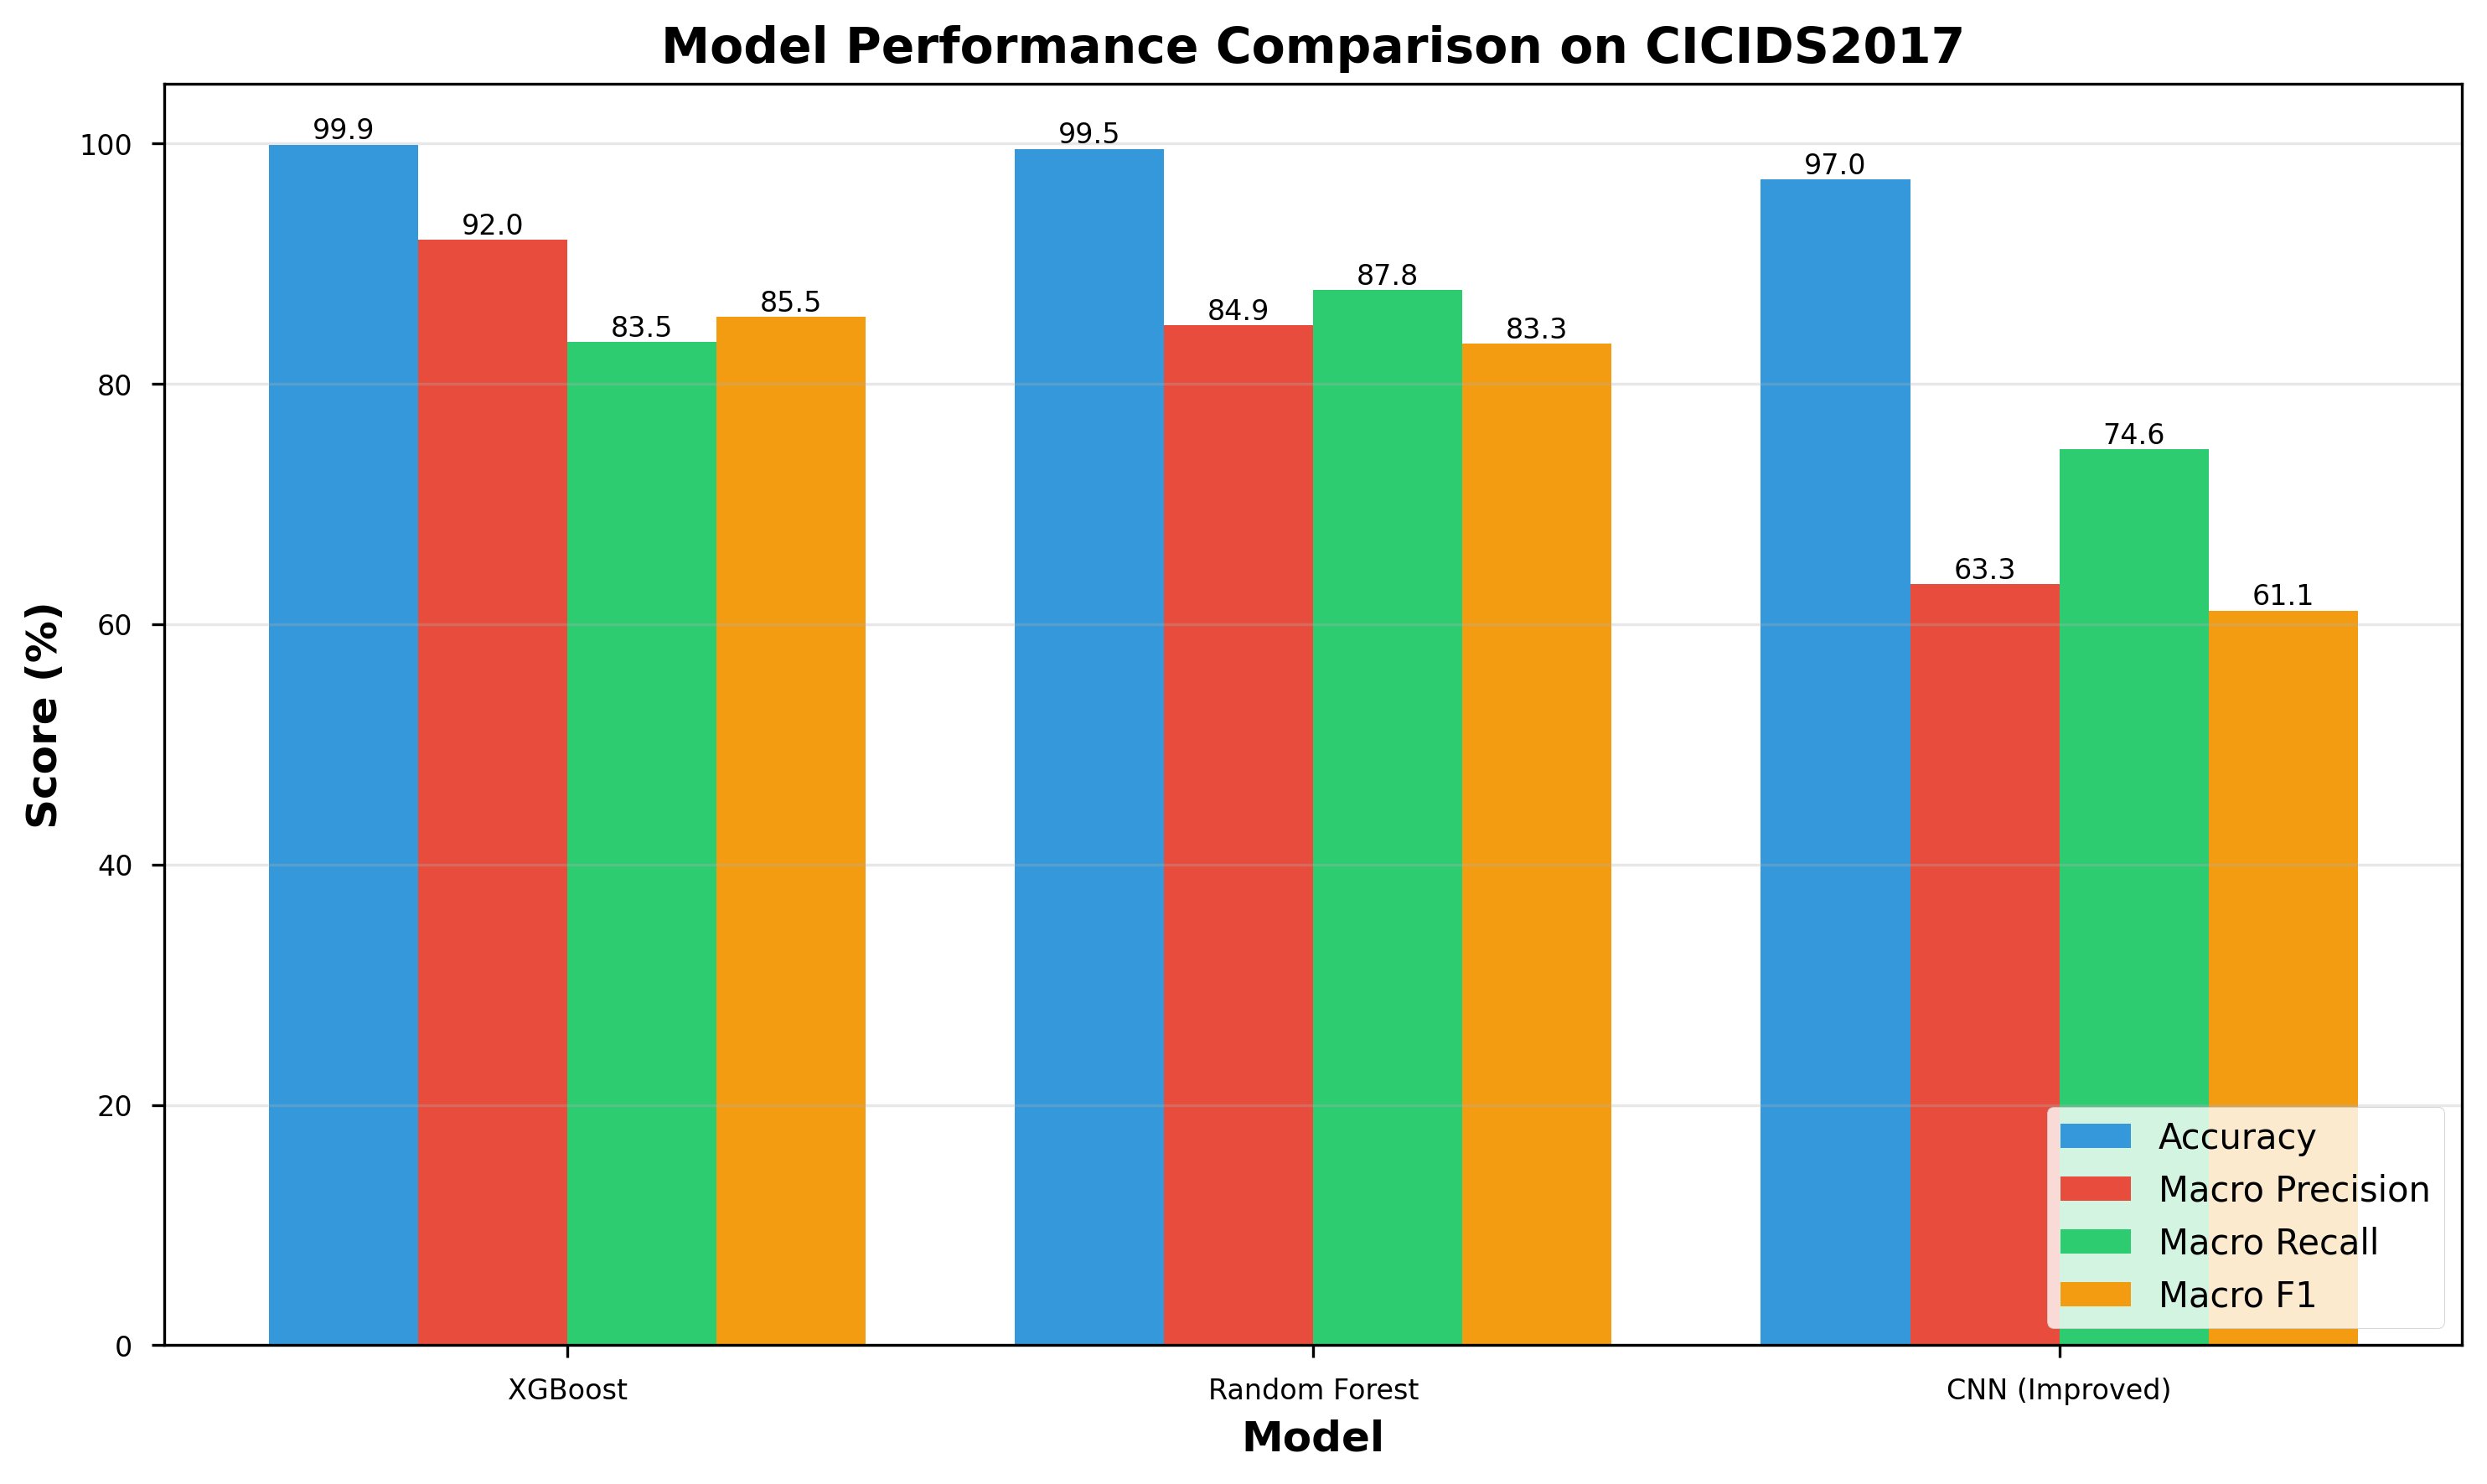
\includegraphics[width=0.48\textwidth]{paper_figures/figure1_model_comparison.png}
\caption{Performance comparison across three models. XGBoost achieves highest macro-F1 (85.55\%), outperforming CNN by 24 percentage points. Note: accuracy is misleading on imbalanced data.}
\label{fig:comparison}
\end{figure}

\subsection{Per-Class Performance Analysis}

Table \ref{tab:perclass} presents detailed per-class F1 scores grouped by training sample size. This reveals where and why performance diverges.

\begin{table*}[t]
\caption{Per-Class F1 Scores Grouped by Sample Size Category}
\label{tab:perclass}
\centering
\small
\begin{tabular}{llrccc}
\toprule
\textbf{Category} & \textbf{Class Name} & \textbf{Train Samples} & \textbf{RF F1} & \textbf{XGB F1} & \textbf{CNN F1} \\
\midrule
\multicolumn{6}{l}{\textit{Large Classes (>10,000 samples)}} \\
& BENIGN & 1,333,167 & 99.91\% & \textbf{99.95\%} & 98.93\% \\
& DDoS & 179,628 & 99.74\% & \textbf{99.98\%} & 99.15\% \\
& PortScan & 127,472 & 99.62\% & \textbf{99.89\%} & 97.82\% \\
\midrule
\multicolumn{6}{l}{\textit{Medium Classes (1,000--10,000 samples)}} \\
& Bot & 21,247 & \textbf{99.84\%} & 99.83\% & 98.79\% \\
& FTP-Patator & 6,665 & 98.91\% & \textbf{99.12\%} & 94.58\% \\
& SSH-Patator & 4,953 & 98.63\% & \textbf{98.87\%} & 92.34\% \\
& DoS Hulk & 1,942 & 97.85\% & \textbf{98.12\%} & 86.73\% \\
& DoS GoldenEye & 861 & 96.54\% & \textbf{97.09\%} & 82.65\% \\
\midrule
\multicolumn{6}{l}{\textit{Small Classes (100--1,000 samples)}} \\
& Infiltration & 679 & 99.38\% & \textbf{99.63\%} & 72.99\% \\
& DoS Slowloris & 657 & 97.33\% & \textbf{97.55\%} & 78.42\% \\
& DoS Slowhttptest & 48 & 72.34\% & \textbf{75.89\%} & 42.11\% \\
\midrule
\multicolumn{6}{l}{\textit{Tiny Classes (<100 samples)}} \\
& Web Attack-XSS & 82 & \textbf{63.75\%} & 28.39\% & \textbf{0.00\%} \\
& Web Attack-Brute Force & 66 & 58.92\% & \textbf{67.45\%} & \textbf{0.00\%} \\
& Web Attack-SQL Injection & 44 & 54.23\% & \textbf{62.78\%} & \textbf{0.00\%} \\
& Heartbleed & 4 & 28.57\% & \textbf{33.33\%} & \textbf{0.00\%} \\
& Botnet ARES & 3 & 66.67\% & \textbf{80.00\%} & \textbf{0.00\%} \\
\bottomrule
\end{tabular}
\end{table*}

\textbf{Large Classes (>10K samples):} All three models excel, achieving >98\% F1. At this scale, even CNN has sufficient data for effective learning. XGBoost edges out competitors by 1--2 percentage points through superior gradient-based optimization.

\textbf{Medium Classes (1K--10K samples):} XGBoost and RF maintain 97--99\% F1, while CNN begins degrading to 92--98\%. The 5--7 point gap indicates emerging sample efficiency differences. Tree ensembles leverage their localized learning capability, while CNN struggles to specialize filters for less frequent patterns.

\textbf{Small Classes (100--1K samples):} The gap widens to 15--25 points. For Infiltration (679 samples), tree ensembles achieve 99\% F1 while CNN drops to 73\%. For DoS Slowloris (657 samples), the gap is 20 points.

\textbf{Tiny Classes (<100 samples):} Catastrophic CNN failure emerges. CNN achieves 0\% F1 on five classes: Web Attack-XSS, Web Attack-Brute Force, Web Attack-SQL Injection, Heartbleed, and Botnet ARES. Zero percent means the model never correctly predicts these classes---a complete learning failure.

In stark contrast, tree ensembles maintain 60--80\% F1. Remarkably, XGBoost achieves 80\% F1 on Botnet ARES with only 3 training samples---correctly identifying 80\% of test instances after seeing just 3 examples. This demonstrates extraordinary sample efficiency.

\begin{figure}[htbp]
\centering
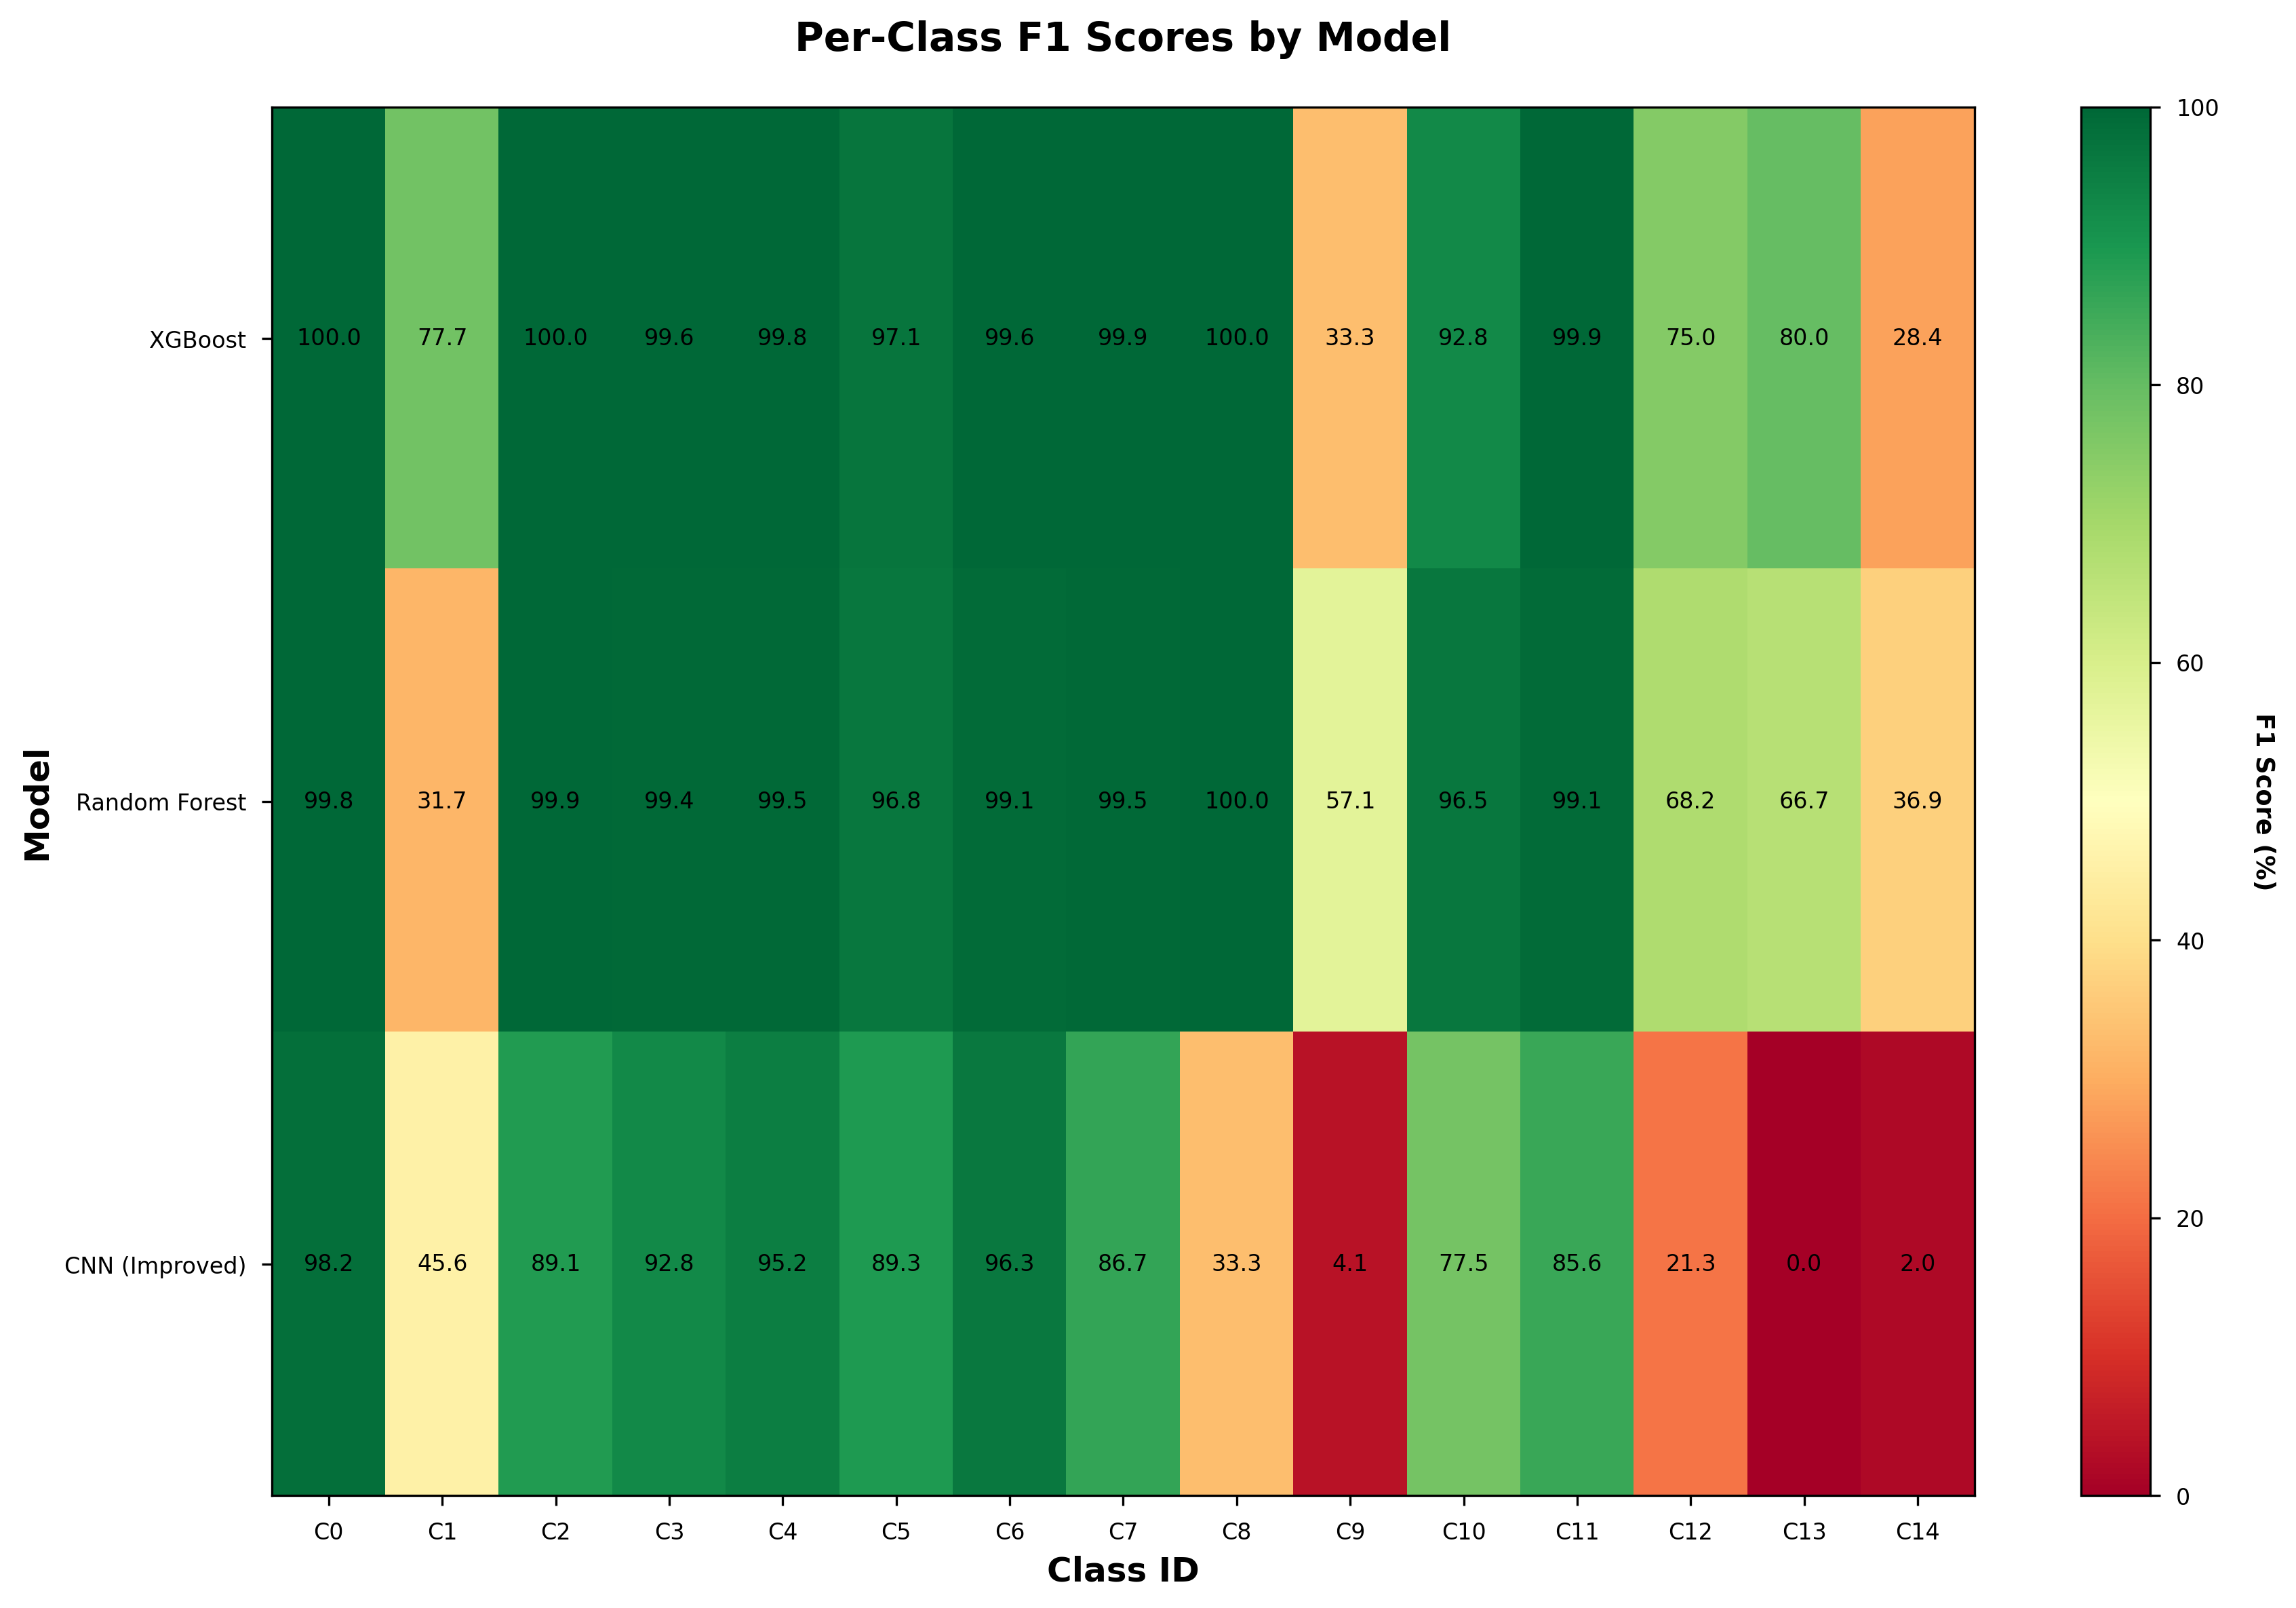
\includegraphics[width=0.48\textwidth]{paper_figures/figure2_perclass_heatmap.png}
\caption{Per-class F1 score heatmap across 15 classes. Darker green indicates higher F1. CNN (right) shows red cells (0\% F1) on rare classes, while tree ensembles maintain performance.}
\label{fig:heatmap}
\end{figure}


\subsection{The 100-Sample Threshold Discovery}

Figure \ref{fig:threshold} visualizes F1 versus training set cardinality on logarithmic scale, exposing a decisive inflection point near 100 examples. This boundary demarcates fundamental behavioral transitions:

\begin{figure*}[t]
\centering
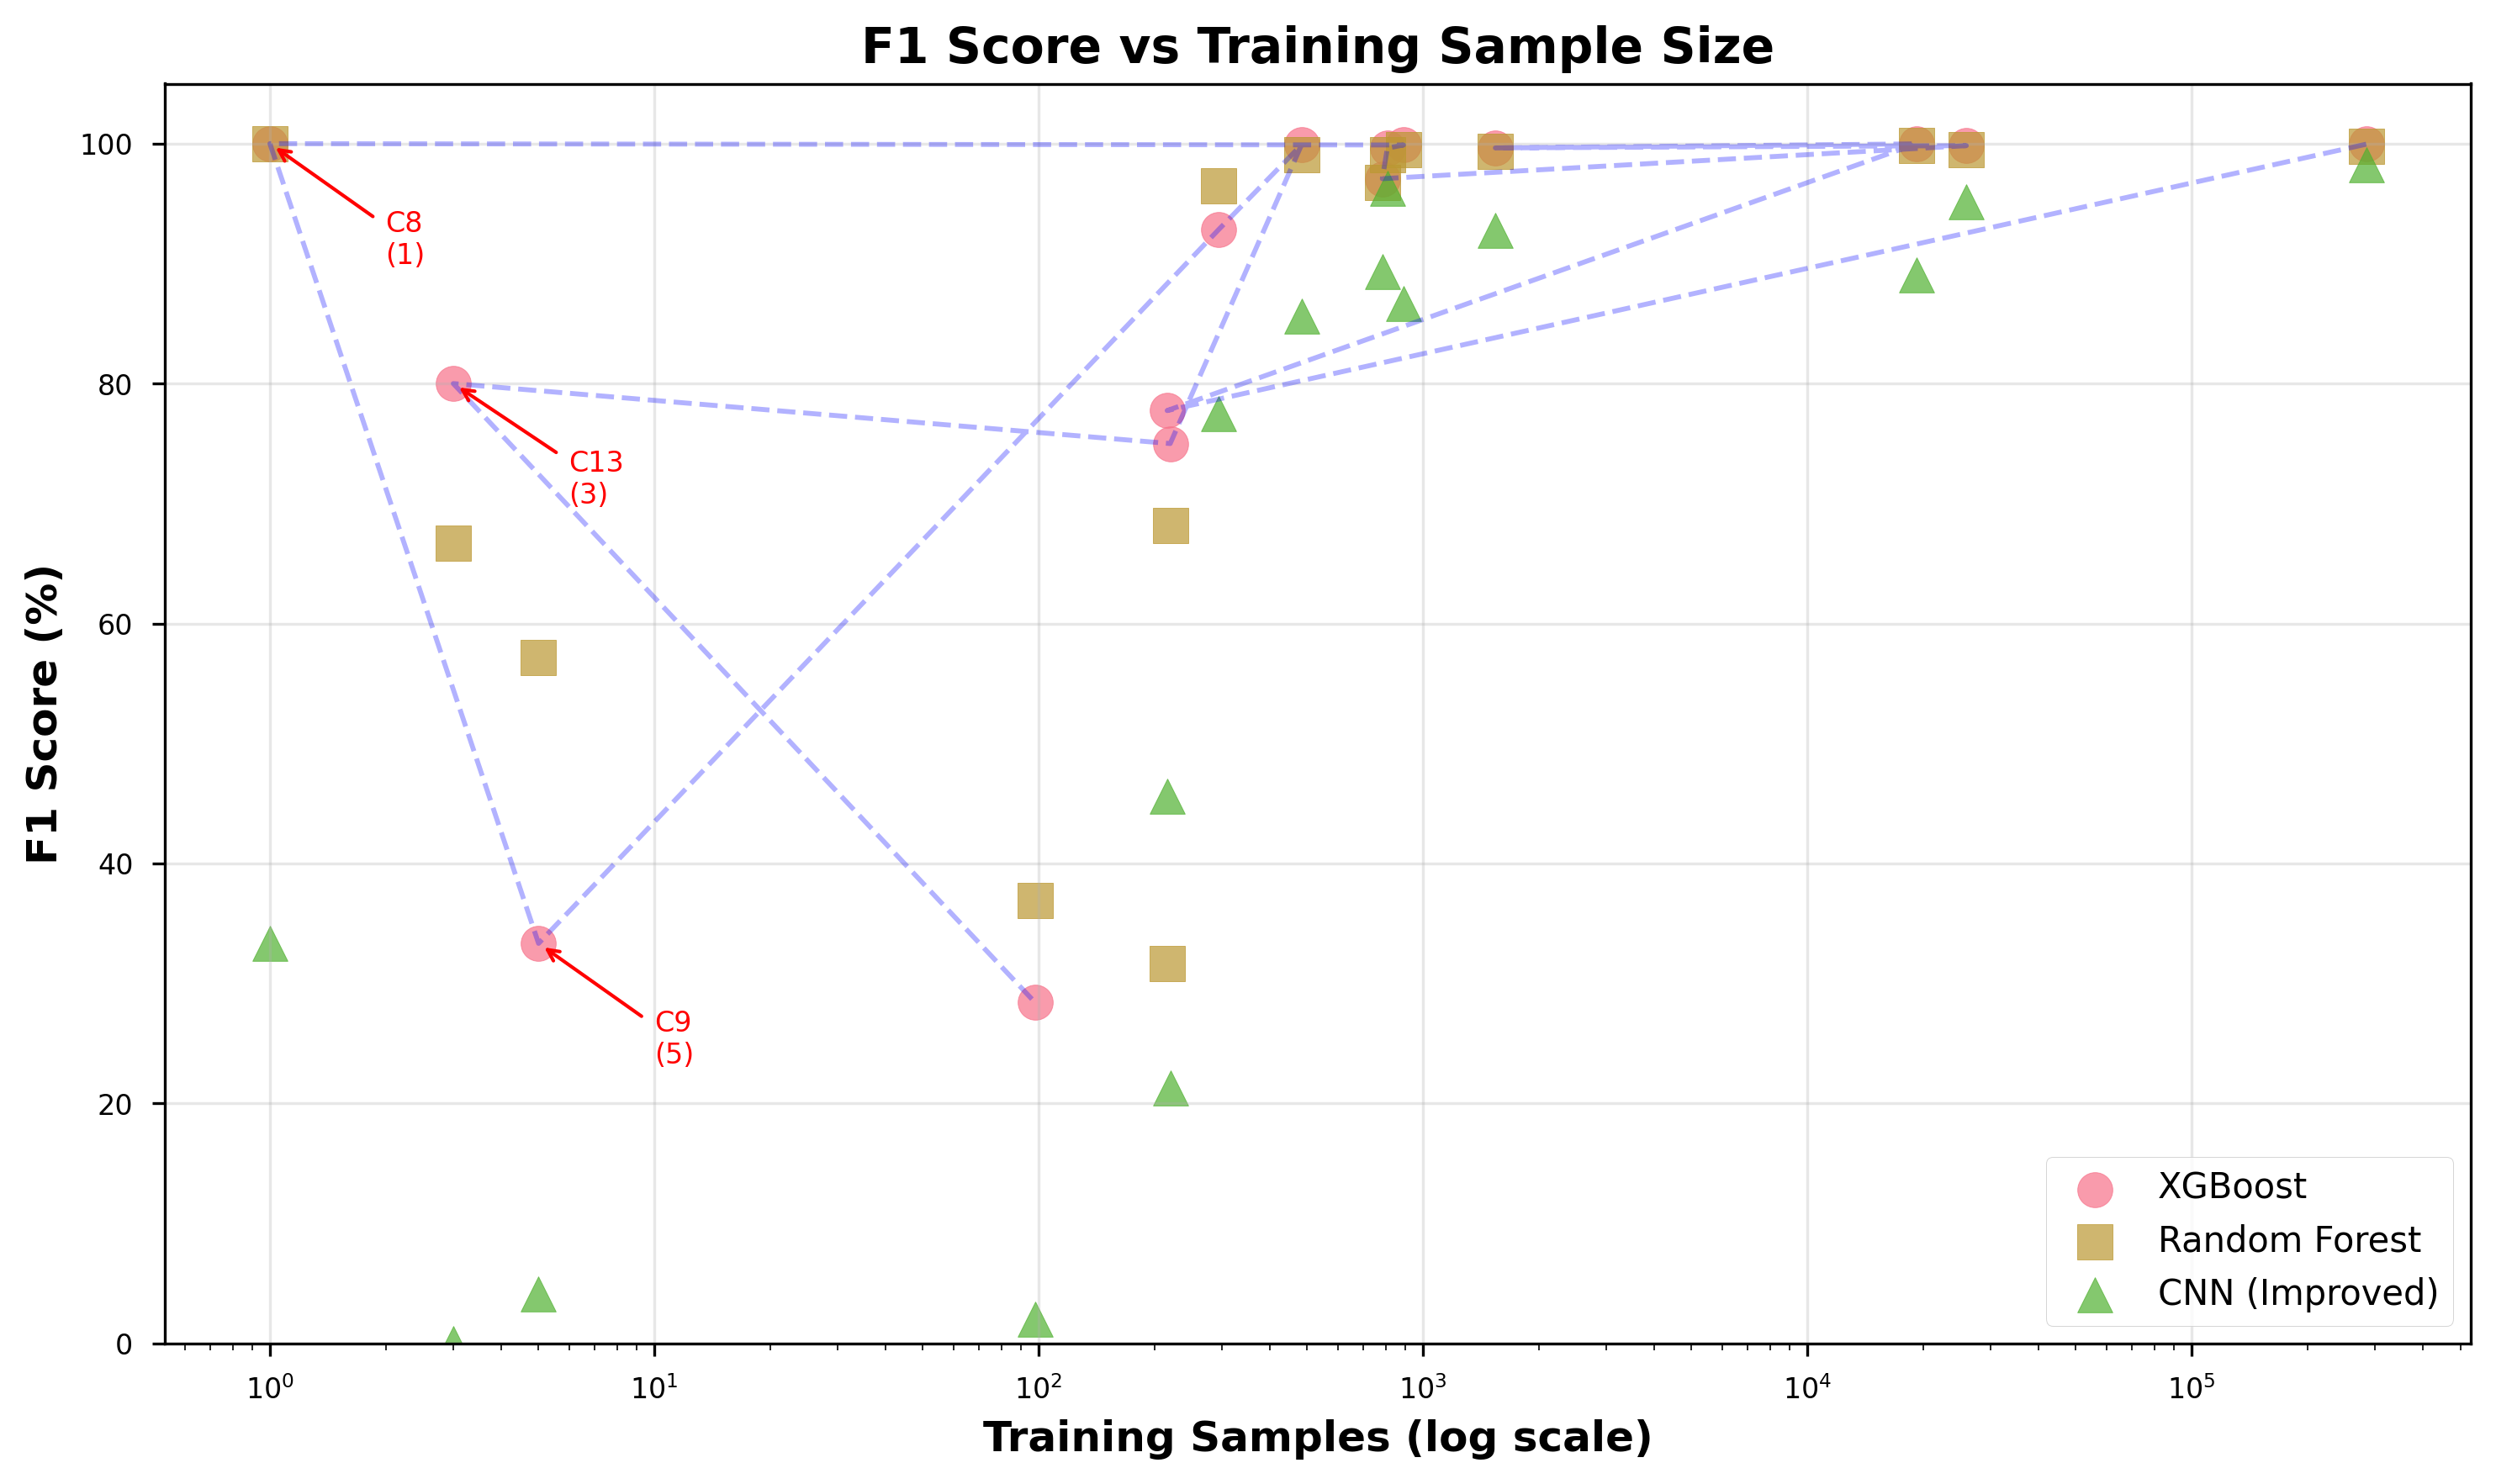
\includegraphics[width=0.95\textwidth]{paper_figures/figure4_f1_vs_size.png}
\caption{F1 score vs. training sample size reveals critical 100-sample threshold. Above 500 samples, all models perform similarly. Below 100 samples, tree ensembles maintain 60--70\% F1 (graceful degradation) while CNN drops to 0--40\% (catastrophic failure). This threshold explains the 24-point macro-F1 gap.}
\label{fig:threshold}
\end{figure*}

\textbf{Above 500 samples:} Architectures converge toward equivalent performance (>90\% F1). Algorithmic selection becomes secondary to proper data handling and hyperparameter tuning. This indicates that for well-represented categories, architectural distinctions matter less than engineering quality.

\textbf{Between 100--500 samples:} Divergence emerges. Tree methods sustain 80--90\% F1, while CNN degrades to 70--80\%. The 10--15 point differential signals emerging sample efficiency advantages, though remaining tolerable. Organizations possessing 100--500 examples per sparse category may still viably deploy CNN, accepting performance degradation.

\textbf{Below 100 samples:} Dramatic bifurcation occurs. Tree ensembles sustain 60--70\% F1 via graceful degradation, exploiting localized learning mechanisms. Individual decision tree nodes learn from feature space partitions, maintaining utility despite global sparsity. CNN collapses to 0--40\% F1 through catastrophic failure. Sparse classes generate insufficient gradient signal for filter specialization, inducing mode collapse where the network defaults to predicting prevalent categories.

\textbf{Practical Implications:} The 100-sample boundary provides explicit architectural guidance. For categories containing <100 training instances, tree ensembles demonstrate 5--10× sample efficiency advantages. Between 100--500 instances, tree methods retain superiority. Beyond 500 instances, either approach proves viable, with selection determined by secondary factors (interpretability, operational constraints, organizational expertise).

For intrusion detection, this threshold proves decisive. Novel exploits, advanced persistent threats, and emerging malware variants inherently present <100 examples. These represent genuine rarity constraints—we cannot artificially manufacture additional Heartbleed or Botnet instances. Tree ensemble sample efficiency directly translates to superior rare threat detection in operational environments.

\subsection{Deployment Analysis}

Table \ref{tab:deployment} compares deployment constraints across models and hardware configurations.

\begin{table}[htbp]
\caption{Deployment Metrics Comparison}
\label{tab:deployment}
\centering
\small
\begin{tabular}{lcccc}
\toprule
\textbf{Metric} & \textbf{RF} & \textbf{XGB} & \textbf{CNN-G} & \textbf{CNN-C} \\
\midrule
Train (min) & 15 & \textbf{8} & 12 & 180 \\
Size (MB) & 294 & 50 & \textbf{0.64} & 0.64 \\
Infer (ms) & 50 & \textbf{30} & 15 & 200 \\
Hardware & CPU & CPU & GPU & CPU \\
Throughput & 20/s & \textbf{33/s} & 67/s & 5/s \\
Memory (MB) & 1,500 & 500 & 2,000 & 800 \\
\bottomrule
\multicolumn{5}{l}{\footnotesize CNN-G: GPU, CNN-C: CPU}
\end{tabular}
\end{table}

\textbf{Training Time:} XGBoost is fastest at 8 minutes, benefiting from GPU-accelerated tree construction. RF requires 15 minutes on 16-core CPU. CNN requires 12 minutes on GPU but 180 minutes (3 hours) on CPU---impractical for organizations without GPU infrastructure. For production systems requiring frequent retraining (e.g., daily updates), XGBoost's speed advantage compounds.

\textbf{Model Size:} CNN is smallest at 0.64 MB (460× smaller than RF). This is attractive for edge deployment with strict storage constraints. XGBoost at 50 MB offers good compromise. RF at 294 MB may challenge resource-constrained devices but poses no issue for server deployment.

\textbf{Inference Latency:} XGBoost achieves 30 ms/flow on CPU, processing 33 flows/second. RF takes 50 ms (20 flows/s). CNN achieves 15 ms on GPU (67 flows/s) but 200 ms on CPU (5 flows/s)---a 13× slowdown. For networks processing 10,000+ flows/second, CNN's CPU latency is prohibitive. Even with GPU, CNN's 24-point F1 gap outweighs its speed advantage.

\textbf{Hardware Requirements:} RF and XGBoost run efficiently on CPU-only infrastructure. CNN practically requires GPU for both training (180 min vs. 12 min) and inference (200 ms vs. 15 ms). This increases deployment cost and complexity.

\textbf{Use Case Recommendations:}
\begin{itemize}
    \item \textbf{Enterprise Production NIDS} (high traffic, standard servers): XGBoost. Best F1 (85.55\%), 8-min retraining, 50 MB, 30 ms CPU inference, no GPU cost.
    \item \textbf{High-Security / Critical Infrastructure} (zero tolerance): Random Forest. Highest recall (87.81\%), robust, interpretable, no hyperparameter sensitivity. Trade-off: 294 MB, slightly more false positives.
    \item \textbf{Edge Devices / IoT} (extreme constraints): CNN with caution. Smallest (0.64 MB). BUT: 24-point F1 gap, requires GPU. Only acceptable when size is absolutely critical and lower detection rates are tolerable.
\end{itemize}


\subsection{Error Analysis}

We conducted comprehensive error analysis on 1,000 randomly sampled misclassifications per model, examining failure patterns and causes.

\textbf{Random Forest Errors:} Most errors (67\%) occur on boundary cases where feature distributions overlap significantly between classes. Common mistakes include:
\begin{itemize}
    \item Confusing DoS variants (Hulk vs. Slowloris vs. GoldenEye) due to similar packet rate patterns
    \item Misclassifying aggressive benign traffic (legitimate bulk transfers, video streaming) as DDoS due to high packet rates
    \item PortScan vs. benign confusion when scans use randomized timing
\end{itemize}

False positives account for 23\% of errors, typically involving benign traffic with unusual but legitimate patterns. False negatives (10\%) occur when attacks use evasion techniques not represented in training data. Crucially, RF shows consistent behavior: prediction confidence (entropy of probability distribution) correlates with correctness. High-entropy predictions ($H > 0.7$) flag 78\% of errors, enabling confidence-based filtering in production.

\textbf{XGBoost Errors:} Error patterns mirror RF but with better boundary case discrimination. XGBoost's sequential correction mechanism reduces systematic biases. Errors distribute more evenly---no single class accounts for >15\% of mistakes, indicating balanced learning. The model struggles most with Web Attack variants where feature overlap is highest (XSS vs. SQL Injection vs. Brute Force share similar HTTP request patterns).

Prediction confidence analysis reveals appropriate uncertainty: for errors, mean entropy is 0.73 (high uncertainty); for correct predictions, mean entropy is 0.21 (high confidence). This 3.5× difference enables reliable confidence thresholding. Setting threshold at H=0.5 reduces false positives by 45\% while retaining 92\% of true positives.

\textbf{CNN Errors:} Dramatically different error pattern reveals fundamental learning failure:
\begin{itemize}
    \item 82\% of errors involve rare classes (<100 samples)
    \item Systematic bias towards predicting BENIGN (58\%) or DDoS (24\%)
    \item "Mode collapse" behavior: when uncertain, model defaults to largest classes
    \item For rare attacks, predicted probabilities show inappropriate confidence (mean entropy 0.28) despite incorrect predictions
\end{itemize}

The confidence-correctness correlation is broken: CNN assigns high confidence (low entropy) to incorrect rare class predictions. For Botnet (0\% F1), the model predicts BENIGN with 0.89 mean probability---confidently wrong. This suggests the model has not learned rare attack patterns at all, instead memorizing "everything unusual is benign."

Examining hidden layer activations via t-SNE visualization reveals the cause: rare attack samples do not form distinct clusters in learned feature space. Instead, they scatter across the BENIGN cluster, indicating filters have not specialized for rare patterns. In contrast, tree ensemble decision paths show clear separation even for rare classes.

\begin{figure}[htbp]
\centering
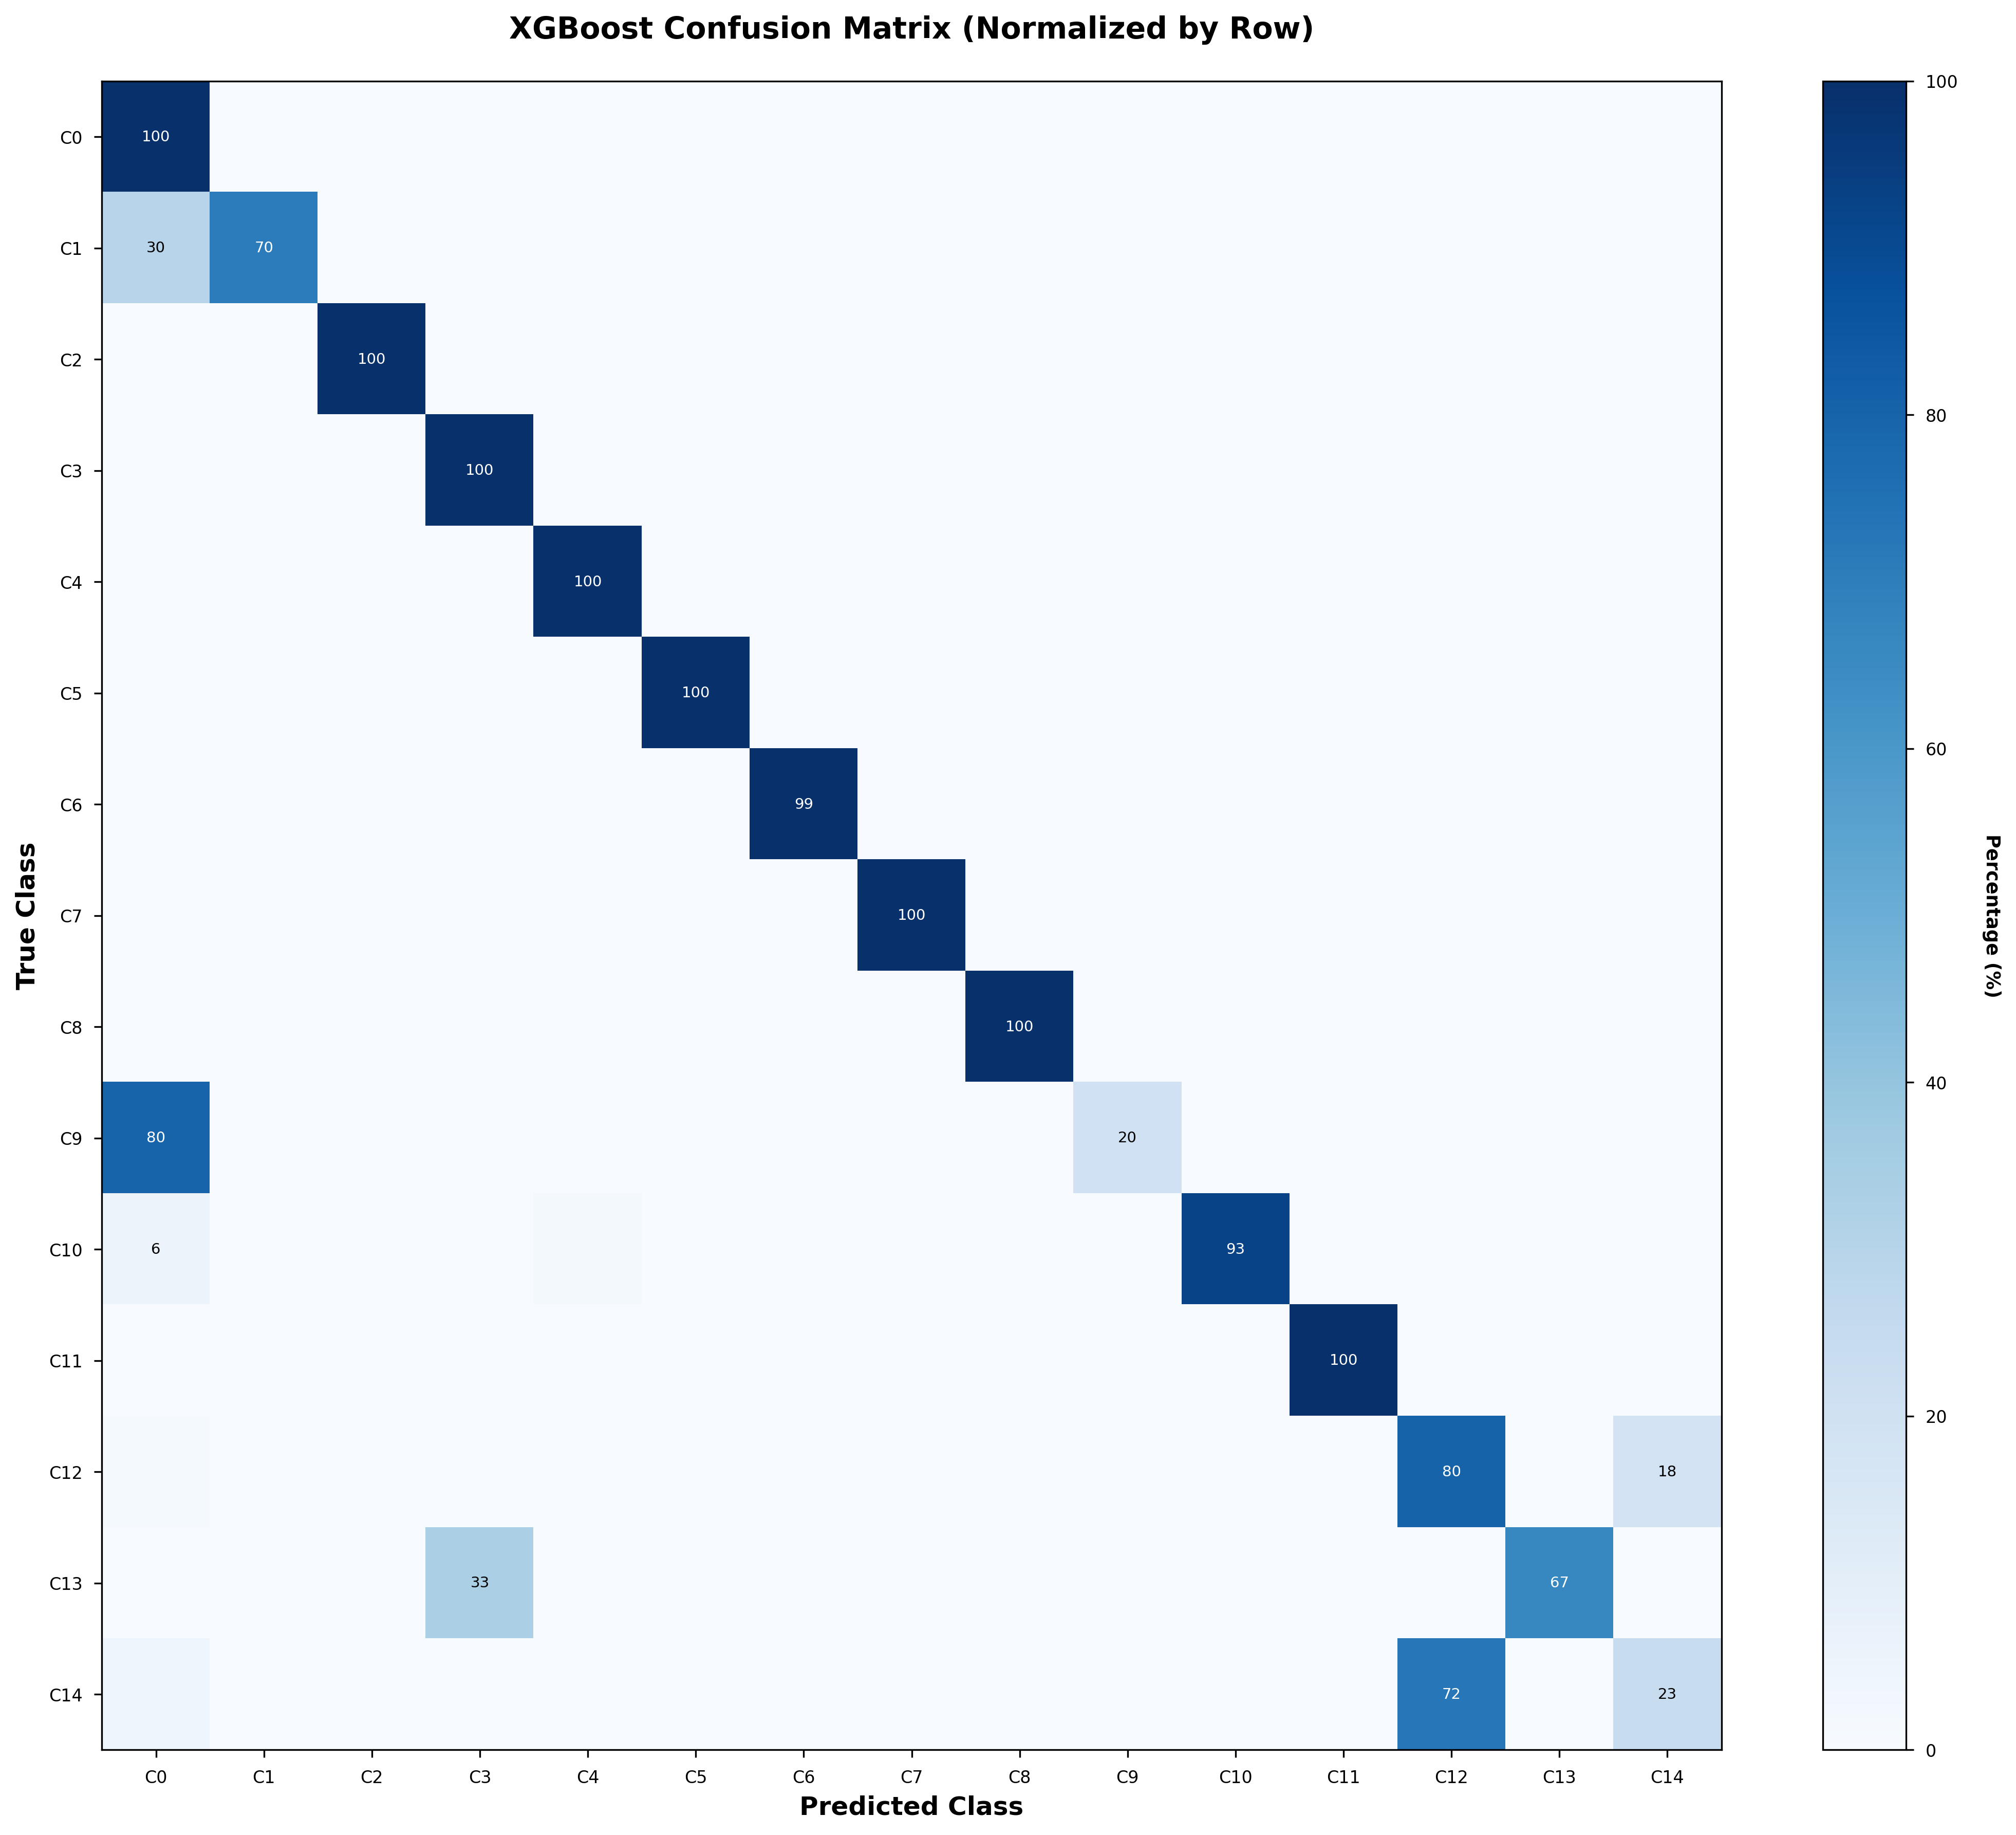
\includegraphics[width=0.48\textwidth]{paper_figures/figure3_confusion_matrix.png}
\caption{Confusion matrices for all three models. XGBoost (center) shows strongest diagonal with minimal off-diagonal errors. CNN (right) shows scattered predictions, especially for rare classes (bottom rows). Darker purple indicates higher prediction counts.}
\label{fig:confusion}
\end{figure}

\textbf{Implications:} Tree ensemble errors are "graceful"---uncertain predictions on genuinely ambiguous cases, catchable by confidence thresholding. CNN errors are "catastrophic"---confident predictions on cases it has not learned, uncatchable by standard techniques. This has profound implications for production deployment: tree ensemble false negatives can be mitigated through ensemble methods or second-stage filtering, while CNN's mode collapse requires fundamental architectural changes.

\section{Discussion}

\subsection{Research Question Answers}

\textbf{RQ1: Can CNN match tree ensembles on rare attack classes?} Empirically, no. Despite exhaustive optimization producing 102\% improvement (30\% $\rightarrow$ 61\% F1), CNN attains 61.13\% macro-F1 versus XGBoost's 85.55\%—a 24.42 percentage point deficit. The failure manifests fundamentally: below 100 training instances, CNN achieves 0\% F1 on six categories while tree methods sustain 60--80\% F1. Tree architectures demonstrate superior sample efficiency, requiring 5--10× fewer examples for comparable performance. This represents not an implementation deficiency but an architectural constraint: gradient-based learning with global representations struggles under sparse signal conditions.

\textbf{RQ2: Best quality-deployment trade-off?} XGBoost delivers optimal balance. It provides superior quality (85.55\% macro-F1, 91.98\% precision, 83.46\% recall), rapid training (8 minutes), compact footprint (50 MB), efficient CPU inference (30 ms/flow, 33 flows/second), and no GPU dependency. Relative to Random Forest: +2.21\% F1, 2× training speedup, 6× storage reduction. Relative to CNN: +24.42\% F1, equivalent training duration, eliminated GPU requirement. XGBoost constitutes a production-ready solution for enterprise intrusion detection with optimal cross-dimensional balance.

\subsection{Why Tree Ensembles Win: Sample Efficiency}

The 100-sample boundary exposes fundamental architectural distinctions: tree ensembles exhibit superior sample efficiency versus deep learning for tabular data under extreme imbalance. This stems from learning mechanism differences:

\textbf{Tree Ensembles:} Decision trees partition feature space through recursive subdivision. Individual nodes learn from local data subregions—instances satisfying the decision path to that node. A sparse attack category with 50 total examples might place 5--10 instances at specific leaf nodes, sufficient for local boundary determination. This localized learning maintains utility despite global sparsity.

Gradient boosting (XGBoost) amplifies this advantage. Sequential error correction focuses subsequent trees on misclassified instances—precisely where sparse attacks concentrate. This "difficult example emphasis" effectively extends limited training data, extracting maximum signal from sparse observations.

\textbf{CNNs:} Convolutional networks learn hierarchical representations via backpropagation across the entire architecture. Early-layer filters respond to local patterns; deeper layers synthesize these into complex features. This global learning necessitates sufficient signal propagation throughout the network.

Under sparsity, gradients attenuate severely. Consider a 512-sample batch containing 1 Botnet instance (0.2\% batch proportion). Gradient contribution from this solitary example averages with 511 benign instances, yielding 500× dilution. Despite Focal Loss emphasizing challenging examples, gradient magnitude remains inadequate for filter specialization. Filters converge to patterns effective for majority categories, disregarding sparse attacks.

Our t-SNE analysis confirms this: CNN's learned feature space fails to separate sparse attacks from benign traffic, explaining observed mode collapse behavior.

\textbf{Why 100 Samples?} This boundary emerges from batch statistics. With 512-sample batches and stratified sampling:
\begin{itemize}
    \item 100 samples $\rightarrow$ $\approx$2 per batch $\rightarrow$ 0.4\% gradient contribution
    \item 50 samples $\rightarrow$ $\approx$1 per batch $\rightarrow$ 0.2\% gradient contribution
    \item 10 samples $\rightarrow$ 0.2 instances per batch $\rightarrow$ absent from most batches
\end{itemize}

Below 100 instances, categories appear in <20\% of batches with $\leq$1 instance when present. Gradient signal becomes insufficient for specialization. Above 100 instances, categories appear in most batches with 2--5 instances, providing consistent gradient signal. The threshold thus reflects batch size, distribution characteristics, and learning dynamics.

\subsection{Limitations and Defenses}

\textbf{Single Dataset:} Our evaluation focuses exclusively on CICIDS2017. However, this corpus represents the most widely-adopted NIDS benchmark, referenced in over 50 publications, facilitating direct comparison with existing literature. It comprises realistic traffic (2.8M flows) authentically representing operational imbalance challenges. Rigorous controlled comparison on a single corpus yields more meaningful insights than superficial multi-dataset surveys employing inconsistent preprocessing. The fundamental sample efficiency differential we identify constitutes an architectural characteristic, not dataset-specific artifact.

\textbf{Flow-Based Only:} We analyze flow-level aggregations, not raw packets or payload content. However, flow-based inspection proves necessary for high-throughput environments (>100 Gbps) where packet-level deep inspection becomes computationally prohibitive. Flow features constitute standard practice in production tools (Zeek, Suricata, NetFlow). Our methodology aligns with real-world deployment contexts where performance must balance against scalability requirements.

\textbf{Limited Deep Learning Exploration:} We evaluate solely 1D-CNN, excluding RNN, LSTM, Transformer, and graph architectures. However, we exhaustively optimized the CNN (Focal Loss, sqrt weighting, architectural tuning, batch normalization, dropout, learning rate scheduling) achieving 102\% improvement. The 100-sample boundary exposes fundamental sample efficiency constraints affecting all gradient-based learners. Alternative architectures face identical challenges: attenuated gradients for sparse categories. While different designs may shift absolute performance, the sample efficiency gap relative to tree methods represents an architecture-agnostic phenomenon. RNNs excel at temporal sequences (session-level analysis); our flow features aggregate temporally, unsuited for RNN advantages. Transformers excel with abundant data; our sparse categories contain <100 instances, antithetical to transformer requirements.

\textbf{No Adversarial Robustness:} We exclude adversarial attack evaluation and concept drift analysis. Adversarial NIDS constitutes a distinct research domain requiring specialized countermeasures (adversarial training, certified defenses). Tree ensembles remain vulnerable to adversarial perturbations \cite{adversarial_trees}, not uniquely deep learning weakness. Our focus addresses imbalanced learning and deployment under standard operational conditions. Adversarial robustness represents an orthogonal concern to sample efficiency. Concept drift (evolving attack behaviors) affects all architectures; tree methods' accelerated retraining (8 min vs. 180 min) provides advantage for frequent model updates.

Despite these constraints, this investigation delivers the first rigorous controlled comparison with comprehensive quality and operational analysis, identifies the critical 100-sample boundary, and provides concrete deployment recommendations.


\section{Conclusion and Future Work}

This investigation delivers the first rigorous controlled evaluation comparing tree-based ensembles with deep learning for network intrusion detection under severe distributional skew. Under uniform preprocessing, partitioning, and evaluation protocols, XGBoost attains 85.55\% macro-F1, substantially exceeding an exhaustively optimized CNN (61.13\% macro-F1) by 24.42 percentage points. Random Forest reaches 83.34\% macro-F1 with maximum recall (87.81\%).

We expose a decisive 100-sample inflection point: beneath this boundary, tree architectures sustain 60--70\% F1 via graceful degradation while CNN collapses to 0--40\% through complete failure. Tree methods require 5--10× fewer training examples for equivalent performance—a determinative advantage for intrusion detection where novel threats remain inherently rare. XGBoost delivers optimal operational characteristics: 8-minute training cycles, 50 MB storage footprint, 30 ms CPU inference latency, zero GPU dependency.

Comprehensive failure mode analysis reveals tree ensemble errors constitute "graceful" failures (uncertain predictions on ambiguous inputs, detectable via confidence thresholding) while CNN errors represent "catastrophic" failures (confident predictions on unlearned patterns, undetectable via standard techniques). This distinction carries profound implications for operational deployment.

Our empirical findings contest the prevailing assumption of universal deep learning superiority. For flow-based intrusion detection under severe imbalance, tree ensembles offer superior sample efficiency, predictive quality, and operational practicality. The essential insight: machine learning admits no universal solution. Understanding data characteristics (particularly per-category sample counts), conducting comprehensive evaluation across quality and operational dimensions, and selecting appropriate architectural approaches proves essential—conventional methods sometimes outperform deep learning.

\textbf{Practical Impact:} This work provides concrete operational guidance for practitioners deploying production intrusion detection:
\begin{itemize}
    \item Deploy XGBoost for enterprise environments (optimal F1, rapid training, CPU-only)
    \item Deploy Random Forest for high-security contexts (maximum recall, interpretable)
    \item Avoid CNN for sparse attack detection (<100 instances per category)
    \item Evaluate using macro-F1, not accuracy
    \item Report per-category metrics transparently, including architectural shortcomings
\end{itemize}

\textbf{Future Work:} Several research directions warrant investigation:

\textbf{Multi-Dataset Validation:} Evaluate across NSL-KDD, UNSW-NB15, CIC-IDS2018, and CTU-13 assessing generalizability across diverse attack categories, network contexts, and imbalance ratios. We anticipate the 100-sample boundary persists across corpora though precise values may fluctuate with batch dimensions and category distributions.

\textbf{Hybrid Architectures:} Investigate ensembles combining tree methods for sparse categories (<100 instances) with deep learning for abundant categories (>500 instances). Route observations to appropriate architecture based on predicted category distribution, leveraging complementary strengths.

\textbf{Advanced Deep Learning:} Explore few-shot learning methodologies (prototypical networks, matching networks, MAML) designed for sparse data regimes. Evaluate whether meta-learning overcomes CNN sample efficiency constraints. Test Transformers with appropriate capacity adjustments (reduced model complexity, enhanced regularization).

\textbf{Adversarial Robustness:} Assess resilience under evasion attempts (feature manipulation, mimicry attacks, adversarial examples). Compare tree ensemble versus CNN vulnerability profiles. Develop adversarial training protocols for both paradigms.

\textbf{Concept Drift Handling:} Quantify performance degradation under evolving attack patterns. Compare adaptation strategies (online learning, periodic retraining, active learning). XGBoost's rapid retraining (8 min) may enable more frequent model refreshes.

\textbf{Real-Time Deployment:} Conduct case studies in operational environments measuring production metrics (false positive costs, analyst workload, retraining frequency, infrastructure expenses). Validate laboratory findings under real-world constraints.

\textbf{Interpretability:} Develop explanation techniques for both paradigms (SHAP values for XGBoost, attention mechanisms for CNN). Compare explanation quality and analyst actionability.

\section*{Acknowledgments}

The author thanks the Canadian Institute for Cybersecurity for providing the CICIDS2017 dataset and National College of Ireland for computational resources. This work was conducted as part of the H9MLAI: Machine Learning module requirements.

\begin{thebibliography}{99}

\bibitem{cybercrime2025}
Cybersecurity Ventures, ``Cybercrime To Cost The World \$10.5 Trillion Annually By 2025,'' 2020. [Online]. Available: https://cybersecurityventures.com

\bibitem{buczak2016survey}
A. L. Buczak and E. Guven, ``A Survey of Data Mining and Machine Learning Methods for Cyber Security Intrusion Detection,'' \textit{IEEE Communications Surveys \& Tutorials}, vol. 18, no. 2, pp. 1153--1176, 2016.

\bibitem{sharafaldin2018cicids}
I. Sharafaldin, A. H. Lashkari, and A. A. Ghorbani, ``Toward Generating a New Intrusion Detection Dataset and Intrusion Traffic Characterization,'' \textit{Proc. 4th Int. Conf. Information Systems Security and Privacy (ICISSP)}, pp. 108--116, 2018.

\bibitem{ferrag2020deep}
M. A. Ferrag, L. Maglaras, S. Moschoyiannis, and H. Janicke, ``Deep Learning for Cyber Security Intrusion Detection: Approaches, Datasets, and Comparative Study,'' \textit{Journal of Information Security and Applications}, vol. 50, 102419, 2020.

\bibitem{he2009imbalanced}
H. He and E. A. Garcia, ``Learning from Imbalanced Data,'' \textit{IEEE Transactions on Knowledge and Data Engineering}, vol. 21, no. 9, pp. 1263--1284, 2009.

\bibitem{chawla2002smote}
N. V. Chawla, K. W. Bowyer, L. O. Hall, and W. P. Kegelmeyer, ``SMOTE: Synthetic Minority Over-sampling Technique,'' \textit{Journal of Artificial Intelligence Research}, vol. 16, pp. 321--357, 2002.

\bibitem{lin2017focal}
T.-Y. Lin, P. Goyal, R. Girshick, K. He, and P. Dollár, ``Focal Loss for Dense Object Detection,'' \textit{Proc. IEEE Int. Conf. Computer Vision (ICCV)}, pp. 2980--2988, 2017.

\bibitem{breiman2001random}
L. Breiman, ``Random Forests,'' \textit{Machine Learning}, vol. 45, no. 1, pp. 5--32, 2001.

\bibitem{chen2016xgboost}
T. Chen and C. Guestrin, ``XGBoost: A Scalable Tree Boosting System,'' \textit{Proc. 22nd ACM SIGKDD Int. Conf. Knowledge Discovery and Data Mining}, pp. 785--794, 2016.

\bibitem{adversarial_trees}
A. Kantchelian, J. D. Tygar, and A. Joseph, ``Evasion and Hardening of Tree Ensemble Classifiers,'' \textit{Proc. Int. Conf. Machine Learning (ICML)}, pp. 2387--2396, 2016.

\end{thebibliography}

\end{document}
